\documentclass[11pt,a4paper]{article}
\usepackage[T1]{fontenc} 
\usepackage[utf8]{inputenc}
\usepackage[english]{babel} 
\usepackage{graphicx}
\usepackage{hyperref}
\usepackage{booktabs}
\usepackage{geometry}
\usepackage{microtype}
\usepackage{parskip}
\usepackage{minted}
\usepackage{pgfplots}
\pgfplotsset{compat=1.18}
\usepackage[syle=ieee]{biblatex}
\addbibresource{ref.bib}
\geometry{margin=2.5cm}

\newcommand{\techterm}[1]{\texttt{#1}}
\newcommand{\supervisor}[1]{\texttt{#1}}
\title{\textbf{Leveraging Honeypots for Threat Hunting}}

\author{
\textbf{Authors} \\ Hugo Jonsson \& Julius Enquist
\\ \\
\textbf{Supervisors} \\ Anders Karlsson, Oleksii Baranovski and Alexandr Silonosov
}

\begin{document}
\begin{figure}[t]
    \centering
    
\includegraphics[width=0.4\linewidth]{img/bthnotext.pdf}
\end{figure}
\maketitle
\date{}

\newpage
\begin{abstract}
    Gaspot\cite{GasPotGithub} and Honeypots (Qeeqbox)\cite{QeeqboxHoneypotsGithub} were deployed with public IP's in order to hunt for active threats. Their collective findings were that....
\end{abstract}

\newpage
\tableofcontents
\newpage

\newpage
\section{Introduction}
This project focuses on the implementation of a comprehensive security environment designed for threat hunting and proactive defense within a public network segment. The core purpose of the assignment is to build a system that moves beyond simple monitoring by enabling the active mitigation of identified threats. By exposing the infrastructure to a public IP subnet, the project allows for the observation of authentic attack campaigns in a controlled laboratory environment.

\subsection{Project Objectives}
The primary goal of this exercise is to simulate a professional security workflow where data collection leads directly to defensive action. The project is structured around several core technical requirements:

\begin{itemize}
    \item Selecting and deploying a customized monitoring stack consisting of a SIEM platform and a Network Intrusion Detection System
    \item Implementing two distinct honeypots to attract and log malicious traffic from the internet
    \item Executing a continuous data collection phase over a period of at least two weeks
    \item Identifying seven significant Indicators of Compromise from the captured logs
    \item Developing and applying custom rules to actively block the sources of these attacks
\end{itemize}

\subsection{Methodology and Scope}
The work involves monitoring traffic through a core switch port to capture data from a public IP subnet. This approach ensures that the gathered information represents actual threats currently active on the internet. By analyzing this data, the project aims to bridge the gap between simple detection and the implementation of a functional defense strategy.

The final stage of the assignment requires verifying the local findings against global intelligence databases. This process ensures that the identified threats are accurately mapped to recognized attack frameworks. The ultimate result is a closed loop security process where evidence from the honeypots is used to strengthen the overall posture of the network through targeted blocking rules.

\subsection{Material}
\label{sec:material}
The experimental setup included the following components:

\begin{itemize}
\item Two computers designated for honeypot deployment.
\item One computer serving as the monitoring system, hosting the Suricata Intrusion Detection System (IDS) and the Wazuh Manager. This system was equipped with two Network Interface Cards (NICs) and is referred to as the \textit{Server} in this report.
\item A Cisco Catalyst 2960 Switch.
\item Access to egress traffic through the BTH Core Switch.
\end{itemize}

All machines operated on Ubuntu Desktop 24.04.4 LTS with default installation configurations.


\newpage
\section{Setup and Installation}

The setup described in this section was implemented using the hardware and systems presented in Section~\ref{sec:material}. Two separate computers were used to deploy the honeypots in order to simplify configuration and maintain physical separation between monitoring and attack surfaces.

The monitoring computer hosted both Suricata IDS and the Wazuh Manager. One NIC (enp2s0) was configured to monitor network traffic from the honeypot environment, allowing Suricata to inspect packets and detect suspicious activity. The second NIC (eno1) was used for management access and communication with other components of the system.
\subsection{Software Configuration}
\begin{itemize}
    \item \textbf{Wazuh}
    \\ Wazuh was configured to recieve local alerts from both Agent: 'Abbe 1' and 'Abbe 2'. That way local alerts are directly sent to the Wazuh Manager. Including both Agent Hosts within VLAN 103 as well as adding their respective IP's, exposed the Agents to the Manager meaning the alerts could be monitored. 
    
    \item \textbf{Suricata IDS}
    \\ Suricata was installed on the main server to perform deep packet inspection on all traffic entering the honeypot network. The configuration involved setting the network interface to promiscuous mode to ensure the capture of all mirrored traffic from the SPAN port. The team modified the \techterm{suricata.yaml} file to define the \techterm{HOME\_NET} variable which included the specific IP addresses of both honeypot hosts. To integrate the system with the SIEM the \techterm{eve.json} output was enabled as the primary log source. This file was then monitored by the Wazuh manager through a localfile entry in the \techterm{ossec.conf} configuration. This setup allowed the manager to parse network alerts and display them in the central dashboard for analysis during the data collection phase.
    
    \item \textbf{Honeypots}
    \\ \textbf{Gaspot}\cite{GasPotGithub} was deployed on Abbe 1. It is a honeypot simulating Veeder-Root Guardian AST tank gauges, with randomized instances that behave like realistic industrial control systems.  
    \\ \textbf{Qeeq: HoneyPots}\cite{QeeqboxHoneypotsGithub} were deployed on Abbe 2. It provides multiple types of honeypots supporting various protocols, including SSH, FTP, HTTP(S), IMAP, and SMTP.  
    
    \item \textbf{Wireguard}
    \\ WireGuard was implemented on the Wazuh Manager to provide a secure encrypted tunnel for remote administrative tasks. The setup process included generating unique public and private key pairs for each device to ensure that only authorized users could establish a connection. The team configured the service to listen on a specific UDP port and adjusted the system firewall (UFW) to permit this traffic. To optimize the connection split tunneling was utilized so that only traffic intended for the lab subnet traveled through the VPN while all other traffic remained on the local network of the user. This configuration enabled stable and secure management of the monitoring stack throughout the duration of the project.
    
    \item \textbf{UFW - Server}
    \\ Uncomplicated Firewall was configured to enforce a restrictive security policy on the Wazuh Manager. By setting the default policy to deny all incoming traffic and only allowing specific necessary services the team ensured a reduced attack surface for the server. Port 1514 and port 1515 were opened specifically for the IP addresses 193.11.189.37 and 193.11.189.38 as these were required for the Wazuh agents to communicate and enroll with the server. Access to port 22 was restricted to the 10.66.65.0/24 subnet to ensure that SSH management was only possible through the secure VPN local network. Finally port 51820 was permitted from any source to facilitate the encrypted WireGuard VPN service which provided remote access to the entire monitoring environment.
    
\begin{figure}[h]
    \centering
    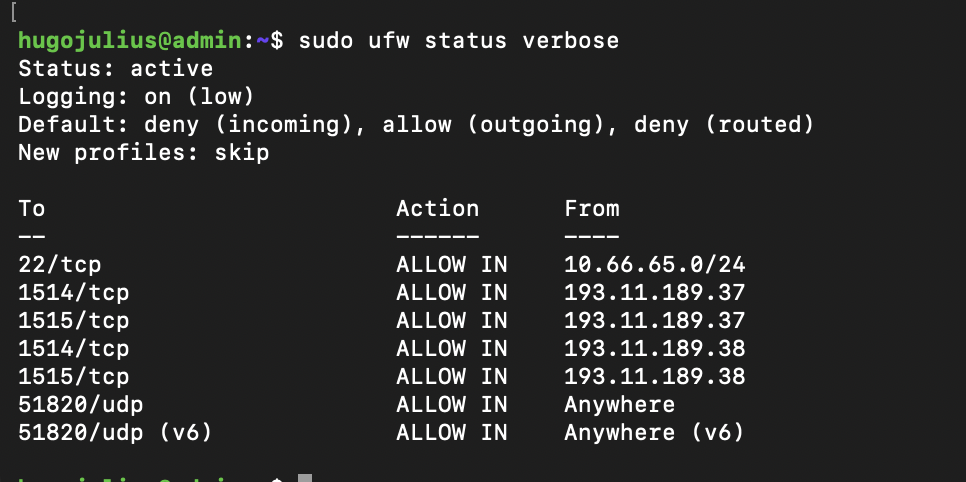
\includegraphics[width=0.8\linewidth]{img/UFWstatus.png}
    \caption{UFW configuration}
    \label{fig:placeholder}
\end{figure}
    
\end{itemize}

\subsection{Switch Configuration}
The Cisco Catalyst 2960 switch was configured as the foundational security layer for the project. By implementing Layer 2 security features the team ensured that only authorized hardware could interact with the honeypot environment.

\textbf{VLAN Segmentation and Port Assignment} \\
The network was segmented using \techterm{VLAN 103} which was assigned to the primary interfaces including the Wazuh Manager on \techterm{Fa/05} and the honeypots on \techterm{Fa/11} and \techterm{Fa/12}. The uplink to the BTH infrastructure was established via the Gigabit interface \techterm{Gi/0/1}. This logical grouping ensured that all traffic related to the experiment remained isolated from the default management VLAN.

\textbf{Port Security and Identity Persistence} \\
To prevent unauthorized devices from connecting to the lab network the team enabled \textbf{Port Security} on all active access ports. The configuration utilized the \techterm{sticky} keyword to automatically learn and lock the MAC address of the connected equipment. Specifically the first honeypot on port \techterm{Fa/11} was locked to the address \texttt{78e3.b5c6.0afc} while the second honeypot on port \techterm{Fa/12} used the address \texttt{78e3.b5c6.0851}. The Wazuh Manager on \techterm{Fa/05} was similarly locked to the address \texttt{e069.95e5.ff7d}. Any attempt to connect a different device would trigger a violation policy set to \textit{restrict} which drops unauthorized traffic while logging the event.

\textbf{Traffic Mirroring and Bandwidth Throttling} \\
A local monitor session was established to facilitate deep packet inspection by the Suricata IDS. The switch was configured to mirror all bidirectional traffic from the source ports \techterm{Fa/11} and \techterm{Fa/12} to the destination port \techterm{Fa/02}. To ensure that the monitoring port would not become overwhelmed the team restricted the speed of the honeypot interfaces to 10 Mbps while maintaining full duplex operation. This intentional throttling provided sufficient headroom for the 100 Mbps monitoring interface to capture and log every packet during high volume attack periods.

\textbf{IP Source Guard and ARP Integrity} \\
The team implemented \textbf{IP Source Binding} to prevent IP spoofing within the subnet. By creating manual bindings for the authorized IP addresses the switch verified that every packet matched its preassigned address. This mechanism worked in tandem with Dynamic ARP Inspection to ensure that malicious actors could not perform man in the middle attacks or hijack the identities of the honeypots during the two week data collection phase.

\newpage
\section{Network Layout and Topology}
The subnet 193.11.189.32/28, which contains public addresses, was provided. Not all IPs were used, as they were unnecessary. Five switch ports were configured with the following details:

\begin{table}[h]
\centering
\caption{Network connectivity and interface specifications}
\begin{tabular}{@{}llllll@{}}
\toprule
\textbf{Host} & \textbf{IP Address} & \textbf{Host Port} & \textbf{Speed} & \textbf{Destination Host} & \textbf{Destination Port} \\ \midrule
Wazuh Manager & 193.11.189.35/28 & eno1 & 100 Mbps & Cisco Catalyst 2960 & Fa/05 \\
Wazuh Manager & Monitoring & enp2s0 & 100 Mbps & Cisco Catalyst 2960 & Fa/02 (SPAN) \\
GasPot Abbe 1 & 193.11.189.37/28 & enp5s0 & 10 Mbps & Cisco Catalyst 2960 & Fa/11 \\
HoneyPots Abbe 2 & 193.11.189.38/28 & enp5s0 & 10 Mbps & Cisco Catalyst 2960 & Fa/12 \\
BTH Core Switch & 193.11.189.0/27 & Fa/11 & 1000 Mbps & Cisco Catalyst 2960 & Gi/0/1 \\ \bottomrule
\end{tabular}
\end{table}

The network topology was designed to allow dedicated traffic flow to the Honeypot hosts while ensuring that management and alert traffic could reach the IDS securely, isolated from general network exposure. This configuration minimizes the risk of direct access to the monitoring infrastructure while maintaining full visibility of network events.

\begin{figure}[h]
    \centering
    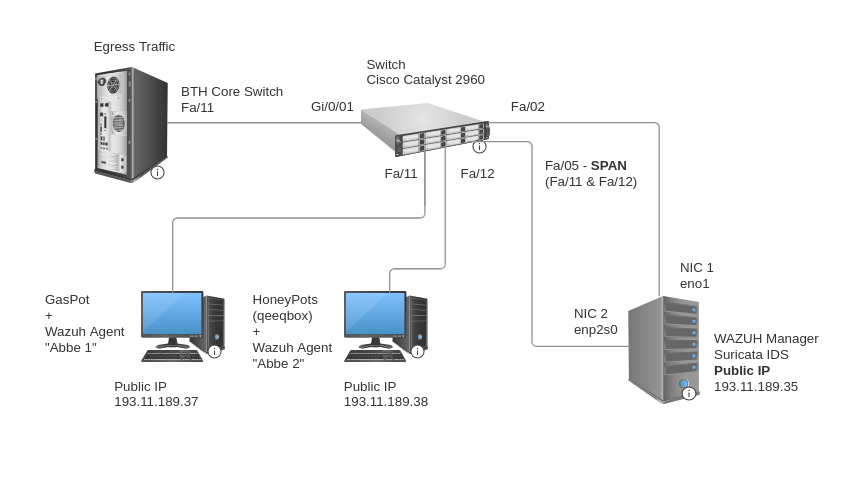
\includegraphics[width=1\linewidth]{img/Topology.png}
    \caption{Network Topology}
    \label{fig:placeholder}
\end{figure}

\newpage
\section{Traffic}
Our collected data shows that traffic...
majority spam
random scanning lookups

\subsection{Grouped by Country}
Create pichart from the list of malicious ips
talk about it
If a country is related to just one attack attempt or multiple? 

FROM VT by API, own script

\begin{center}
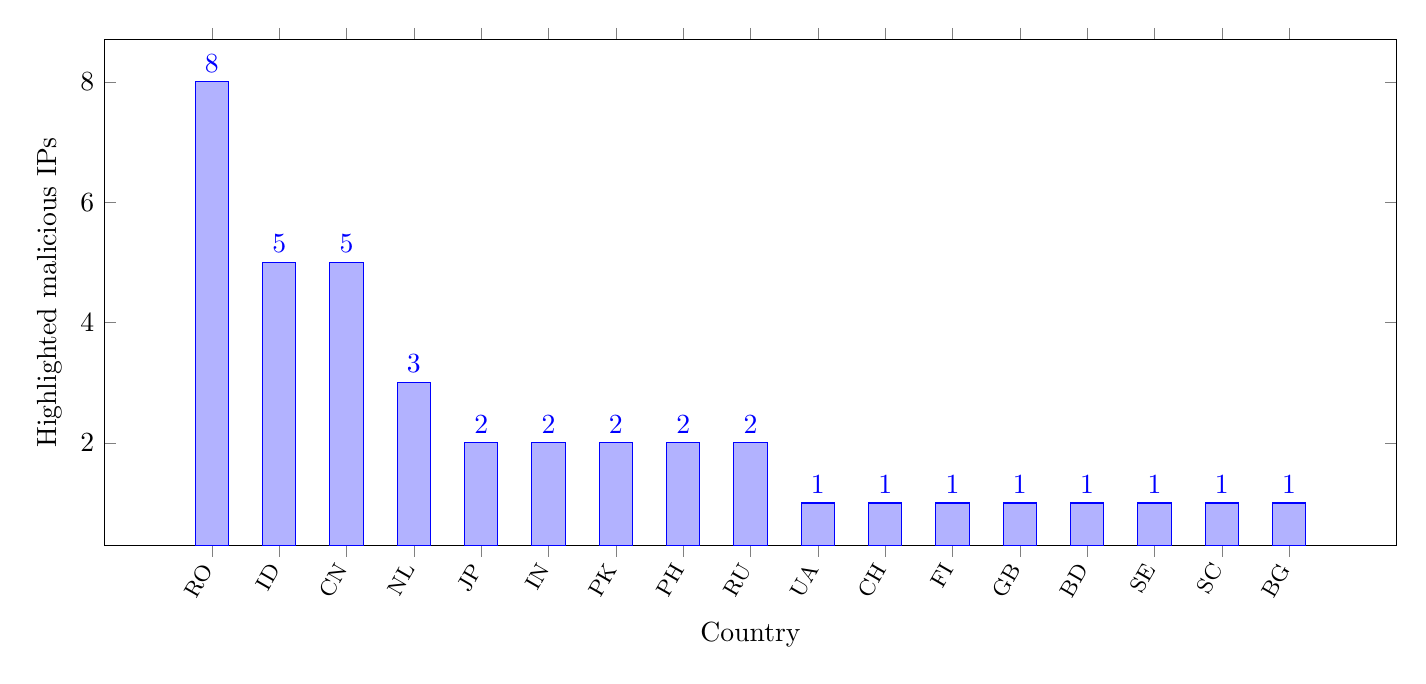
\begin{tikzpicture}
\begin{axis}[
ybar,
width=18cm,
height=8cm,
symbolic x coords={RO,ID,CN,NL,JP,IN,PK,PH,RU,UA,CH,FI,GB,BD,SE,SC,BG},
xtick=data,
xlabel={Country},
ylabel={Highlighted malicious IPs},
nodes near coords,
bar width=12pt,
x tick label style={
rotate=60,
anchor=east,
font=\footnotesize
}
]
\addplot coordinates {
(RO,8) (ID,5) (CN,5) (NL,3) (JP,2) (IN,2) (PK,2) (PH,2) (RU,2) (UA,1) (CH,1) (FI,1) (GB,1) (BD,1) (SE,1) (SC,1) (BG,1) 
};
\end{axis}
\end{tikzpicture}
\end{center}


\subsection{Grouped by Network}
Show piechart for ips
Talk about how many might be bot's from different ips performing same scans.
same subnets?
Botnets could be based in Romania.


\subsection{Alerts}
Our definition of an alert is based on Suricata's update ruleset\cite{suricata-update}. Within this update the ruleset we used \textbf{Emerging Threats Open} as our.
Talk about how suricata might define levels of threat and the scale of this project. These 2 might not be suitable and might needed adjustments.

\newpage
\section{Our 7 Highlighted Alerts}

\subsection{Alert 1}
Rule level 13, word info

The Alert showing IoC:
\inputminted[
fontsize=\footnotesize,
breaklines,
frame=lines
]{json}{alerts/Level 13.json}



\newpage
\subsection{Alert 2: EternalBlue Probe (Generic Flags)}
\textbf{Rule Level:} 9 \\
\textbf{Signature:} \texttt{ET EXPLOIT Possible ETERNALBLUE Probe MS17 010 (Generic Flags)} \\
\textbf{Description:} 
This alert identifies a general attempt to probe the system for the MS17 010 vulnerability by looking for specific anomalies in the SMB packet headers. The Generic Flags designation suggests that the traffic originated from a broad automated scan or a custom script rather than a specific exploitation framework. This type of activity represents the constant background noise of the internet where botnets continuously search for unpatched systems to infect with malware or ransomware.

\begin{center}
\textbf{Associated IP's}
\end{center}

\begin{table}[h]
\centering
\begin{tabular}{|c|c|}
\hline
120.89.64.93 & 103.3.220.228 \\ \hline
218.205.64.41 & 123.108.93.66 \\ \hline
122.52.203.208 & 182.10.130.147 \\ \hline
115.187.30.154 & 36.77.254.203 \\ \hline
203.135.57.98 & 82.208.111.237 \\ \hline
103.132.231.115 & 103.155.184.106 \\ \hline
103.178.112.91 & 103.207.4.145 \\ \hline
\end{tabular}
\caption{Associated IP Addresses}
\end{table}

The Alert showing IoC:
\inputminted[
fontsize=\footnotesize,
breaklines,
frame=lines
]{json}{alerts/Eternal Blue Gen.json}



\newpage
\subsection{Alert 3: EternalBlue Probe (MSF Style)}
\textbf{Rule Level:} 9 \\
\textbf{Signature:} \texttt{ET EXPLOIT Possible ETERNALBLUE Probe MS17 010 (MSF style)} \\
\textbf{Description:} 
Unlike the previous alert this signature specifically matches the traffic fingerprint of the Metasploit Framework which is a professional tool used for penetration testing and exploit delivery. Seeing this alert confirms that the honeypot is being targeted by tools capable of full system exploitation. The MSF style probe is more focused and indicates that the attacker is using a standardized environment to verify the vulnerability before potentially launching a more destructive payload like an encrypted ransomware attack.

\begin{center}
\textbf{Associated IP's}
\end{center}

\begin{table}[h]
\centering
\begin{tabular}{|c|c|}
\hline
120.89.64.93 & 103.3.220.228 \\ \hline
218.205.64.41 & 123.108.93.66 \\ \hline
122.52.203.208 & 182.10.130.147 \\ \hline
115.187.30.154 & 36.77.254.203 \\ \hline
203.135.57.98 & 82.208.111.237 \\ \hline
103.132.231.115 & 103.155.184.106 \\ \hline
103.178.112.91 & 103.207.4.145 \\ \hline
\end{tabular}
\caption{Associated IP Addresses}
\end{table}

The Alert showing IoC:
\inputminted[
fontsize=\footnotesize,
breaklines,
frame=lines
]{json}{alerts/Eternal Blue MSF.json}




\newpage
\subsection{Alert 4: Local File Inclusion Attempt}
\textbf{Rule Level:} 9 \\
\textbf{Signature:} \texttt{ET WEB\_SERVER /etc/passwd Detected in URI} \\
\textbf{Description:} 
This alert identifies a Local File Inclusion attempt targeting the linux operating system password file. By injecting the file path into the Uniform Resource Identifier the attacker hopes to trick the web server into displaying sensitive system information. The password file is a common target because it reveals a list of all user accounts on the machine which is essential for further exploitation such as brute forcing specific accounts. Detecting this signature highlights the ongoing efforts to exploit path traversal vulnerabilities in web applications to gain deeper access to the underlying server environment.

\begin{center}
\textbf{Associated IP's}
\end{center}

\begin{table}[h]
\centering
\begin{tabular}{|c|c|}
\hline
89.42.231.182 & 204.76.203.215 \\ \hline
204.76.203.73 &  \\ \hline
\end{tabular}
\caption{Associated IP Addresses}
\end{table}

The Alert showing IoC:
\inputminted[
fontsize=\footnotesize,
breaklines,
frame=lines
]{json}{alerts/passwd URI.json}



\newpage
\subsection{Alert 5: Remote Command Execution Attempt}
\textbf{Rule Level:} 9 \\
\textbf{Signature:} \texttt{ET WEB\_SERVER /bin/sh In URI Possible Shell Command Execution Attempt} \\
\textbf{Description:} 
This alert identifies a critical attempt to execute arbitrary commands by targeting the system shell via the web interface. The presence of the bin sh string in the Uniform Resource Identifier indicates that an attacker is trying to exploit a command injection vulnerability to gain an interactive command prompt on the server. By attempting to call the shell directly the adversary aims to bypass application logic and run malicious scripts or download additional payloads from a remote server. This type of attack represents a high level of intent as it moves beyond simple reconnaissance into active exploitation with the goal of achieving complete system compromise.

\begin{center}
\textbf{Associated IP's}
\end{center}

\begin{table}[h]
\centering
\begin{tabular}{|c|c|}
\hline
101.36.104.242 & 154.81.14.244 \\ \hline
106.13.183.26 & 194.113.38.28 \\ \hline
114.220.75.156 & 223.199.158.205 \\ \hline
115.190.164.9 & 37.120.213.13 \\ \hline
138.2.0.137 & 82.24.64.32 \\ \hline
83.168.71.160 &  \\ \hline
\end{tabular}
\caption{Associated IP Addresses}
\end{table}

The Alert showing IoC:
\inputminted[
fontsize=\footnotesize,
breaklines,
frame=lines
]{json}{alerts/Possible SH.json}



\newpage
\subsection{Alert 6}
\texttt{data.alert.signature: ET WEB\_SERVER Generic PHP Remote File Include}

\begin{center}
\textbf{Associated IP's}
\end{center}

\begin{table}[h]
\centering
\begin{tabular}{|c|c|}
\hline
101.36.104.242 & 154.81.14.244 \\ \hline
106.13.183.26 & 194.113.38.28 \\ \hline
114.220.75.156 & 223.199.158.205 \\ \hline
115.190.164.9 & 37.120.213.13 \\ \hline
138.2.0.137 & 82.24.64.32 \\ \hline
83.168.71.160 &  \\ \hline
\end{tabular}
\caption{Associated IP Addresses}
\end{table}

\inputminted[
fontsize=\footnotesize,
breaklines,
frame=lines
]{json}{alerts/PHP Include.json}



\newpage
\subsection{Alert 7}
\texttt{data.alert.signature: ET REMOTE\_ACCESS MS Remote Desktop Administrator Login Request}

\begin{center}
\textbf{Associated IP's}
\end{center}

\begin{table}[h]
\centering
\begin{tabular}{|c|c|}
\hline
2.57.121.22 & 5.181.86.60 \\ \hline
80.94.95.83 & 80.94.95.43 \\ \hline
80.94.95.224 & 118.193.73.8 \\ \hline
80.66.83.43 & 165.154.10.165 \\ \hline
162.210.245.77 & 2.57.121.21 \\ \hline
80.94.95.221 & 80.66.66.24 \\ \hline
2.57.121.20 & 80.94.95.238 \\ \hline
\end{tabular}
\caption{Associated IP Addresses}
\end{table}

 
The Alert showing IoC:
\inputminted[
fontsize=\footnotesize,
breaklines,
frame=lines
]{json}{alerts/Remote Desktop.json}



\newpage
\nocite{*}
\printbibliography[heading=bibintoc,title={References}]

\end{document}